% 中文阅读稿：由 article/aamas2027/main.tex 翻译而来；不用于 AAMAS 正式投稿。
\documentclass[UTF8,twocolumn]{ctexart}
\usepackage[a4paper,top=1.8cm,bottom=1.8cm,left=1.65cm,right=1.65cm,columnsep=0.65cm]{geometry}
\usepackage{amsmath,amssymb}
\usepackage{booktabs}
\usepackage{array}
\usepackage{graphicx}
\usepackage{url}
\usepackage{natbib}
\usepackage[colorlinks=true,linkcolor=blue,citecolor=blue,urlcolor=blue]{hyperref}
\setlength{\parindent}{2em}
\setlength{\parskip}{0pt}
\emergencystretch=3em
\setcounter{secnumdepth}{3}
\newcommand{\blank}{\textemdash}
\newcommand{\unknown}{\textsc{未知}}
\newcommand{\rare}{\textsc{稀有}}
\newcommand{\Description}[1]{}
\title{知己所长：从情境化同行判断中赢得角色}
\author{匿名作者（中文阅读稿）}
\date{}
\begin{document}
\maketitle
\noindent\textbf{内部预结果中文阅读稿。} 当前科学发布门仍处于关闭状态。下面的表格在确认数据被观察之前定义实验；数值结果单元有意留空。

\begin{abstract}
多智能体系统必须在尚不知道哪位协作者能够使依赖项可用之前分配责任，而下游失败又会把产出方缺陷与接收方集成问题纠缠在一起。现有的声誉、验收和终局奖励方案通常把这些来源合并：它们可以对智能体排序，却无法判断接收方对交付物的具体使用究竟是在说明产出方的问题，还是在说明接收方自身的问题。我们提出“赢得角色”（\emph{earning roles}）：一种责任感知协议，将带版本的交付物绑定到接收方可观察的使用行为，通过责任所有权门过滤，在下一次分派之前发布所得证据，并且只把延迟的、仅针对已选机会的信用更新应用于未来机会。该协议给出一个可证伪预测：在信息、候选集合和完整成本都匹配的条件下，只有当情境化证据在验收结果和终局结果之外增加了可归因于产出方的信息时，它才应当改善对未见过责任的分派。我们形式化事件边界和读取截点，并规定 ArtifactRole 与 PeerSelect 两条评测轨道，配套同信息基线、结构根级划分，以及延迟、遗忘、归因和成本指标；一般性专长、普适声誉和无界的工作流发现不在本文主张范围内。
\end{abstract}

\section{引言}

在具有依赖关系的多智能体工作流中，协作者的价值往往通过另一个智能体尝试使用其产出物的过程来体现。使用其工作的智能体所做的判断，何时、如何能够让协作者赢得未来的责任机会？考虑两个构造出来的队列处理案例：二者具有相同的拒绝结果和相同的团队失败结果。在第一个案例中，产出方违反了优先级模块契约；在第二个案例中，该模块本身正确，但接收方错误地实现了消费者。相同的反馈需要不同的责任分派。只观察拒绝和终局失败无法区分这两个案例；接收方关于自己使用了什么、为何失败的记录，可能提供缺失的证据。

这个例子隔离出责任混淆：同一条反馈可能描述产出方正确性、接收方集成，或二者都不是。接收方直接拥有关于交付物使用的证据，但它的判断也可能反映自身的集成困难。要从这种判断中学习，就必须分离这些来源，并检验所得证据是否能够预测有用的未来分派。后续结果可以影响再后续的决策；但它不能追溯性地改变已经封存的分派在当时可获得的信息。

本文研究一个更尖锐的问题：\emph{实际接收并使用交付物的智能体，何时能够为产出方的未来责任提供可靠证据？} 这个问题有一个不可跳过的顺序：
\begin{equation}
\begin{aligned}
&\text{交付}\rightarrow\text{接收方使用与判断}\rightarrow\text{产出方归因}\\
&\rightarrow\text{未来分派}\rightarrow\text{未见过的质量与成本}.
\end{aligned}
\label{eq:story}
\end{equation}
终局分数本身无法识别究竟是哪一个产出方造成了缺陷。一个验收比特无法区分“产出物有用”和“接收方容易集成”。一个从不改变后续执行前分派的角色后验，也不能称为角色形成。

核心想法是：把接收方的局部观察变成一个公开、绑定版本并带有责任边界的证据对象。只有当交付物被观察到、接收方的动作可以追溯到该交付物，并且契约检查排除了接收方负责的工作时，产出方才获得信用。证据发布不会悄悄触发策略更新。在后续任务开始之前，合法的责任所有者读取状态快照，选择器封存分派及其选择概率。只有在该后续任务具有独立终局结果之后，延迟信用更新才会发生。这样就把“接收方看到了什么”和“未来责任实际产生了什么”分开，并使这种分离在账本中可观察。

图~\ref{fig:overview} 展示了这一闭环；颜色分别表示情境化观察、公共证据和后续决策。

我们将该协议命名为“赢得角色”。这个名称描述的是一个可测量的过程：协作者通过可归因的证据，在固定的信息和成本契约下改变未来分派，从而赢得责任机会。我们称这种证据为责任感知的角色证据（responsibility-aware role evidence，RARE）；这个名称指向闭环的证据语义，而不是某一种更新器。RARE 由“判断--归因--分派”闭环定义，而不是由某种表示、神经网络头、RLS 更新或周期性重拟合定义。要检验的科学主张是：与原始验收、仅终局结果和同信息情境信任相比，这一闭环能够识别有用的角色证据。

本文提出四项可检验的设计贡献：
\begin{itemize}
  \item 我们定义事件和信息契约，分离产出方质量、接收方动作、下游采用、最终结果和 \unknown{}，同时保留精确的交付物、版本、读取截点和选择概率。
  \item 我们给出两阶段角色证据协议：证据发布是不可变的，不会改变策略；后续分派在执行前封存；延迟的、仅针对已选机会的信用更新只能影响它所评估的未来机会。这些边界使非干扰性和幂等重放可被检验。
  \item 我们规定用于责任诊断的 ArtifactRole 轨道和次级 PeerSelect 机制轨道，并配套匹配的基线、结构根级划分，以及完整资源核算，从而区分信息价值和闭环团队收益。
  \item 我们明确可证伪边界：如果接收方证据没有样本外信息、同信息信任基线能够解释效果、归因不安全，或在匹配的完整成本下质量收益消失，则角色形成主张不通过。
\end{itemize}

\begin{figure*}[t]
\centering
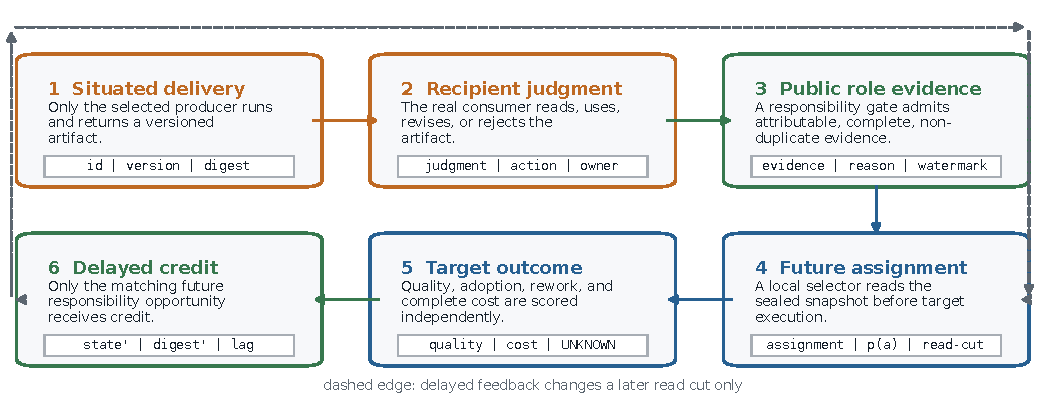
\includegraphics[width=\textwidth]{figures/overview.pdf}
\caption{赢得角色协议。橙色表示情境化观察；绿色表示可归因于产出方的证据，而“未知”分支仅用于审计；蓝色表示已经封存的分派和评分结果。灰色虚线反馈是延迟的、仅针对已选机会的反馈，它进入未来状态和下一次读取截点，但不改变历史证据或已经封存的分派。同行关系边仅用于描述，不表示因果关系。}
\Description{协议图展示了同行关系、产出方交付物及接收方使用、接收方信号和路径证据、归因进入产出方所有证据或仅用于审计的未知分支、带版本的角色账本、读取截点、探索后封存的分派、独立评分的结果，以及进入未来状态和下一次读取的延迟且仅针对已选机会的反馈。}
\label{fig:overview}
\end{figure*}

当前证据边界是有意设置的。开发阶段的追踪记录只验证协议的部分边界，并暴露了评分器和责任归属方面的失败；因此，下面的主张仍然绑定于独立冻结的实验及其证据等级。本文余下部分依次说明研究缺口，定义事件和信息契约，规定协议和匹配比较，给出研究问题、预留结果矩阵、当前证据和局限。

\section{相关工作与定位}

与本文问题最接近的工作在三个轴上有所不同：观察了什么、状态何时变化，以及哪一方的贡献获得信用。表~\ref{tab:novelty} 将这一边界明确列出。协作者选择和声誉方法启发了自适应选择，图结构和角色系统启发了组织变化；但这些工作本身都没有识别某个具体产出方的交付物是否造成了接收方的动作。一个情境信任或延迟老虎机适配器提供的是同信息的强基线，而不是本文所提机制的同义词。

\begin{table*}[t]
\centering\scriptsize
\setlength{\tabcolsep}{3.2pt}
\begin{tabular}{p{0.16\textwidth}p{0.22\textwidth}p{0.19\textwidth}p{0.17\textwidth}p{0.17\textwidth}}
\toprule
代表性方法与问题 & 观察信号与更新 & 责任/信用语义 & 实验对象 & 本文差异/检验内容 \\
\midrule
Curiosity-Driven Partner Selection；Defection at First Sight \cite{leung2025partner,russell2026partner} & 交互结果；社会博弈反馈之后改变伙伴状态 & 同行层面的交互收益；所引公式没有暴露产出方--接收方产出物门 & 约定或困境博弈 & 带版本的交付物使用和产出方归因 \\
Reputation as a Solution to Cooperation Collapse \cite{ren2026reputation} & 共享评价和合作历史；汇总声誉更新 & 广义声誉/合作分数；所引公式没有暴露产出方和接收方所有权字段 & 语言智能体社会协作 & 公共的责任安全证据和显式 \unknown{} \\
AgentNet；GPTSwarm \cite{yang2025agentnet,zhuge2024gptswarm} & 智能体轨迹、图结构或路由结果；组织随时间变化 & 路由/角色效用；所引公式没有定义产出方--产出物信用标签 & 图或工作流协调 & 将接收方动作绑定到一次交付以及未来责任所有者分派 \\
Dynamic Role Assignment；MoRSE \cite{zhang2026dynamic,li2026morse} & 任务上下文和角色/子任务表现；重新分配角色或专家 & 角色/专家效用；所引公式没有暴露接收方集成内部的产出方--产出物归因 & 辩论或混合专家工作流 & 责任门、跨所有者传播和延迟纠正 \\
有限时间多臂老虎机 \cite{auer2002finite} & 已选臂的奖励；观察到臂收益后更新 & 臂层面奖励；没有产出方--接收方所有权契约 & 在观察收益下执行前选择 & 经典的仅选中项控制；情境和延迟适配器需要单独资格验证 \\
\bottomrule
\end{tabular}
\caption{本文使用的创新边界。表中各行是比较家族，并不声称每个来源实现了相同任务。合格的适配器必须保留所列的可见信息、到达顺序、仅选中项分母和完整成本，才能进入科学实验矩阵。}
\label{tab:novelty}
\end{table*}

本文与普通在线学习的区别在于时间和语义。源判断在后续分派之前可用，但后续质量结果只有在该分派执行之后才可用。目标结果到达后可以影响更晚的决策。使用它重构更早的分派会违反当时的可用信息边界；把它当作源产出物的标签，也需要单独的归因论证。我们的协议把两个事件显式分开，并报告维持这种分离所需的服务成本。因此，老虎机估计器是有用的更新比较条件，却不是本文声称的贡献本身。

\section{问题形式化}
\label{sec:problem}

\subsection{对象与信息边界}
在第 $t$ 个事件中，任务提供上下文 $x_t$ 和合法候选集合 $C_t$。选择器必须在 $C_t$ 中任何候选执行之前选择一个候选：
\begin{equation}
 a_t\sim\pi_{\theta}(\cdot\mid x_t,C_t,R_t),\qquad a_t\in C_t,
 \label{eq:choice}
\end{equation}
其中 $R_t$ 是在读取截点 $w_t$ 可获得的公共证据快照。只有被选中的候选会被计入执行成本。该候选生成带版本的交付物 $o_t$ 及摘要 $d_t$；接收方 $j_t$ 读取该交付物并采取动作 $m_t$。接收方可以接受、修改、拒绝，或者无法完成集成。

最小可审计事件为
\begin{equation}
 e_t=(x_t,C_t,a_t,o_t,j_t,J_t,m_t,Q_t,Y_t,\tau_t,c_t),
 \label{eq:event}
\end{equation}
其中 $J_t$ 是接收方判断，$Q_t$ 是产出方契约检查，$Y_t$ 是任务定义的独立后续结果或终局结果，$\tau_t$ 是反馈到达元数据，$c_t$ 是完整成本记录。事件还保存候选版本、任务/结构根标识、产出物摘要、特征模式版本、选择概率 $p_t=\pi_\theta(a_t\mid x_t,C_t,R_t)$、读取截点摘要和证据谱系。

\paragraph{具体实例。} 在队列案例中，$x_t$ 是 JSON 任务请求，$C_t=\{A,B\}$ 是合法产出方菜单，$a_t=B$ 表示选择产出方 $B$。交付物 $o_t$ 是 $B$ 提交的、带摘要 $d_t$ 的带版本优先级模块；接收方字段 $j_t=k$ 记录 $k$ 的导入、测试或修复动作 $m_t$；$Q_t$ 只检查产出方负责的队列和优先级路径；$Y_t$ 是后续消费者结果；$c_t$ 包含模型、工具、token 和墙钟时间成本。

如果对 $k$ 的消费者路径进行了修复，该修复记录在 $m_t$ 中，并将责任门设置为 $G_t=0$，而不改变 $B$ 的产出方证据。

策略只能使用在读取截点之前已经到达的公共事件。隐藏金标准、私有评分器、未来目标结果、另一策略的状态以及未执行候选，都不能影响选择、重试、停止或更新。缺失或不可归因的事件属于 \unknown{}，而不是负标签。这个边界区分了角色信号与方便的事后分数。

\subsection{责任门}
对于源事件，只有同时满足以下条件时才定义 $G_t=1$：（i）产出方契约或预先注册的源缺陷唯一绑定到产出方；（ii）接收方检查了 $o_t$，且其动作可以追溯到 $o_t$；（iii）接收方负责的集成路径为空；（iv）$J_t$、$m_t$、$Q_t$、标识符、版本和摘要完整；（v）该源事件尚未被计入信用。否则 $G_t=0$，该源事件不能创建产出方证据。

这个门区分了四类经常被合并的观察：产出物内容缺陷、接收方自己的集成工作、汇点或最终任务失败，以及无法解决的归因。公共记录保存 $G_t=0$ 的原因。这样就可以测量安全性：拒绝含糊证据的方法可能具有更高的 \unknown{} 率，却产生更少的错误产出方惩罚。

图~\ref{fig:method-state} 展示事件、公共证据和局部决策三条泳道。

\begin{figure*}[t]
\centering
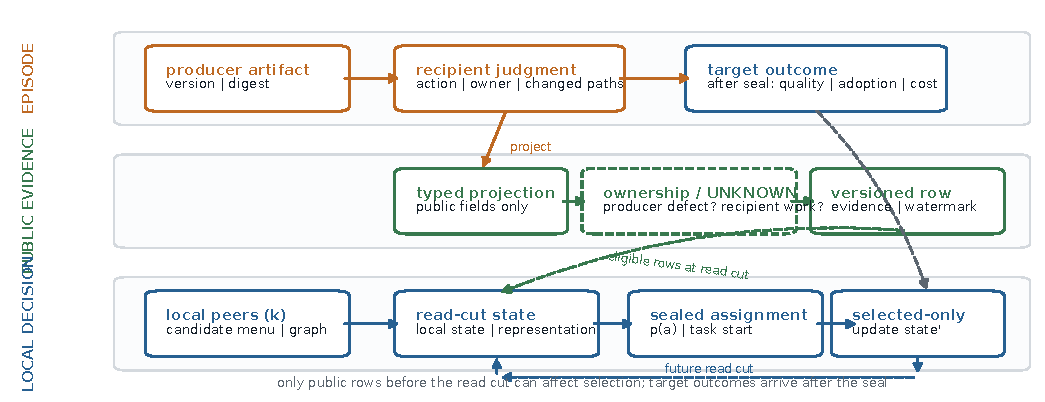
\includegraphics[width=\textwidth]{figures/method_state.pdf}
\caption{从证据到角色状态。事件泳道记录产出方和接收方实际做了什么；公共证据泳道只投影经过类型检查和责任检查的字段；局部决策泳道在读取截点读取可用记录，然后封存分派。目标结果在封存之后到达，只更新相匹配的已选机会。表示和更新器保持可替换。}
\Description{三条水平泳道分别展示事件产出物和判断、经过所有权检查和未知分支的公共证据投影，以及从候选菜单到读取截点状态、封存分派和仅针对已选项更新的局部决策。虚线箭头表示证据何时可用以及目标结果的延迟到达。}
\label{fig:method-state}
\end{figure*}

\section{赢得角色：责任感知协议}
\label{sec:method}

\subsection{两阶段证据与更新}
该协议有两个相互独立的接口：
\begin{align}
 \operatorname{publish}(e_t)&\rightarrow \{\text{RoleEvidence},\;\unknown{},\;\text{invalid}\},\\
 \operatorname{choose}(x_t,C_t,R_t)&\rightarrow (a_t,p_t,\delta_t),\\
 \operatorname{validate}(j_t)&\rightarrow \{\text{credit},\;\unknown{},\;\text{invalid}\},\\
 \operatorname{update}(\text{credit})&\rightarrow \{\text{updated once},\;\text{no-op}\}.
 \label{eq:interfaces}
\end{align}
发布可以改变后续分派的公共输入，但不会调用持久化更新器。对于后续目标分派 $j$，只有在以下条件同时满足时，信用才是合法的：该分派在目标选择和任务启动之前已经写入；被选候选及其选择概率与封存预览一致；目标交付物和结果完整；并且该分派尚未被计入信用。此时更新器评估的是未来责任机会，而不是源事件。

因此，事件时间契约为
\begin{equation}
\begin{aligned}
&\text{源选择}\rightarrow\text{交付}\rightarrow(Q,J,m,Y)\rightarrow G\\
&\rightarrow\text{证据发布}\rightarrow\text{分派}\rightarrow\text{目标结果}\\
&\rightarrow\text{延迟的仅选中项更新}.
\end{aligned}
\label{eq:timeline}
\end{equation}
修正会创建一个更高版本的证据，并且只影响未来快照。重复、迟到、乱序、资源失败或无效事件，要么作为幂等空操作处理，要么显式记录为 \unknown{}。账本重放必须重现相同的状态摘要和选择序列。

\subsection{证据表示与候选评分}
对于上下文 $r$ 中的产出方 $v$，最小公共状态为
\begin{equation}
 R(v,r)=(n(v,r),s(v,r),u(v,r)),
 \label{eq:state}
\end{equation}
其中 $n$ 统计合格证据数量，$s$ 累积责任安全的正/负标签，$u$ 记录未解决或被拒绝的证据。候选分数可以把任务表示 $h(x,v,r)$ 与公共证据项结合起来：
\begin{equation}
 \operatorname{score}(v\mid x,r)=w^\top h(x,v,r)+\beta\frac{s(v,r)}{n(v,r)+\alpha}.
 \label{eq:score}
\end{equation}
对于队列实例，$r$ 是优先级契约上下文，$h(x,B,r)$ 是产出方 $B$ 的固定任务--候选表示，而 $n,s,u$ 是在责任门通过的带版本事件上统计的计数。仅由接收方负责的修复会增加 $u$ 或创建显式 \unknown{} 记录；它不能增加 $B$ 的 $s$。

表示 $h$、更新器和常数是可替换的实现条件，而非科学研究对象。该分数是契约层构造，不是定理，也不主张某一个骨干网络最优。选择器使用预先注册的探索下限，记录 $p_t$，并采用“预览--分派--提交”流程，从而保证写入未来分派时不会重新采样候选。

同一协议产生三个可观察预测。第一，在仅接收方干预下，通过错误产出方归因率和 \unknown{} 率测量责任安全。第二，通过读取截点和分派顺序不变量，以及在选择时不存在目标结果字段，测量时间有效性。第三，通过每事件更新延迟、积压、状态字节数和完整成本，测量受限在线服务能力。这些预测对应 RQ2--RQ4 的终点，并不是分数自动满足的假设。

\subsection{可执行的选择器与更新契约}
该协议可以通过一个小型有状态选择器运行起来，其接口在读取确认数据之前固定。我们只使用冻结的文本编码器，把任务、候选的公共描述和候选的合格证据映射到同一空间；反馈事件不会更新编码器。为了防止某个档案偷偷复用训练决策头的标签，每个候选都有带时间戳的档案快照以及快照之后的证据增量：
\begin{align}
 P_{v,k}&=\operatorname{summarize}\{e_i:G_i=1,\;t_i<\kappa_k\},\\
 D_{v,k,t}&=\operatorname{summarize}\{e_i:G_i=1,\;\kappa_k\leq t_i\leq w_t\},\\
 z_t(v)&=[\phi(x_t)\,\|\,\phi(P_{v,k})\,\|\,\phi(D_{v,k,t})\,\|\,b(v)] .
 \label{eq:selector-state}
\end{align}
这里 $\kappa_k$ 是最近一次档案截点，$w_t$ 是合法读取截点，$\phi$ 是冻结的，$b(v)$ 包含在 $w_t$ 已经公开的版本和不确定性特征。空档案或空增量必须显式表示，不能用未来标签替代。这种拆分是谱系规则，而不是调参约定：一个事件只能进入 $P$、$D$ 或之后的目标结果中的一个。

候选分布为
\begin{equation}
 \begin{aligned}
 q_t(v)&=\operatorname{softmax}_{v\in C_t}\left(g_\psi(z_t(v))\right.\\
       &\qquad\left.+\theta_v^\top\phi(x_t)\right),
       \qquad a_t\sim q_t,
 \end{aligned}
 \label{eq:selector}
\end{equation}
其中 $g_\psi$ 是一个固定的小型头，$\theta_v$ 是每个候选的残差；只有当某个已选分派的独立结果到达之后，$\theta_v$ 才允许改变。头部、温度、探索下限、裁剪规则和学习率都是配置字段，不能在看过确认结果后再选择。实验比较完整状态、仅档案、仅增量、仅残差和无历史版本，因此收益不能仅归因于“融合”这个词。

运行时，选择器执行五项可审计操作。（1）把源判断追加到不可变账本并应用所有权门；被拒绝或不完整的记录变成 \unknown{}。（2）推进读取水位并物化状态快照，记录特征模式和状态摘要。（3）只对合法候选菜单打分，并在目标开始前写入候选集合、概率、采样动作和分派摘要。（4）当目标结果到达时，验证相匹配的分派、仅选中项资格、版本和幂等键。（5）执行一次有界残差更新并发出新的状态摘要；档案和增量的物化等待下一次声明的读取截点。该顺序使服务崩溃之后的事件重放不会改变已经封存的选择。

\begin{table}[t]
\centering\scriptsize
\setlength{\tabcolsep}{2pt}
\caption{状态字段及其合法更新事件。字段只能在列出的截点之后读取，且绝不会追溯性地编辑已经封存的分派。}
\label{tab:state-contract}
\begin{tabular}{p{.25\columnwidth}p{.25\columnwidth}p{.38\columnwidth}}
\toprule
字段 & 来源 & 更新边界 \\
\midrule
档案 $P_{v,k}$ & $\kappa_k$ 之前通过责任门的证据 & 下一次档案截点；此后不可变 \\
增量 $D_{v,k,t}$ & $\kappa_k$ 之后的新证据 & 读取水位 $w_t$ \\
残差 $\theta_v$ & 已选目标结果 $Y_t$ & 仅匹配的延迟更新 \\
不确定性 $u(v)$ & 未知、重复或修正记录 & 单调审计更新 \\
分派 $a_t,p_t$ & 候选菜单和状态快照 & 目标执行前封存 \\
\bottomrule
\end{tabular}
\end{table}

该实现契约给出了在线方法可测量的含义，但没有声称某个编码器或头部普遍最优。它也使困难情况能够执行：迟到的判断改变未来快照；接收方负责的修复不能训练产出方残差；缺失的目标结果不会触发更新。确认实验将从同一本用于审计归因的账本中补充延迟、状态规模和预测效用。如果同信息下的简单校准比较器与完整选择器相匹配，论文将报告协议边界，而不会把收益归因于融合架构。

\subsection{什么才算创新}
本文声称的对象，是这样一个闭环：情境化判断成为可归因证据，证据改变一个合法的未来分派，而该分派产生一个未见过的质量--成本结果。现有表示、冻结编码器、RLS、在线逻辑回归、周期性重拟合、缓存和提示模板都属于实现或比较选择。所需检验包括匹配构成、去掉单个机制的消融、证据内容突变，以及同信息情境控制器。如果这些控制条件复现完整结果，则闭环机制没有可识别的优势。

\section{基准与基线}
\label{sec:benchmark}

\subsection{两条互补轨道}
主轨道 \textbf{ArtifactRole} 是从 TeamBench 派生出的候选基准。它包含产出方交付物、接收方依赖、使用/返工/拒绝动作、责任检查、后续分派、下游采用和完整成本。候选结构根是 DIST1 queue-race（开发诊断）和 PIPE3 stream-processing（有条件的确认）；改名后的种子不算独立结构根。只有在材料可见、写入权限、评分器覆盖、结构根独立性和干净重放都通过之后，才能晋升。

次级 \textbf{PeerSelect} 轨道使用一个固定版本的本地图交互基准，用于研究仅选中项收益、局部候选集、在线更新、漂移和服务成本。它把更新行为隔离在更小的局部选择任务上，但不能证明情境化产出物判断或产出方归因。两条轨道共享事件和选择器接口，同时保持任务、标签、评分器、分母和主张相互独立。

\subsection{预注册基线}
所有主实验臂都获得相同的候选菜单、初始机会、模型/API/工具预算、探索机会、反馈到达计划、失败处理和完整成本核算。每个实验臂只读取其合法历史。表~\ref{tab:baselines} 列出矩阵必须排除的替代解释。
\begin{table*}[t]
\centering\small
\begin{tabular}{p{0.18\textwidth}p{0.38\textwidth}p{0.32\textwidth}}
\toprule
实验臂 & 读取/更新契约 & 所检验的替代解释 \\
\midrule
Uniform & 候选菜单；固定的局部均匀采样 & 随机分配和探索下限 \\
No update & 初始先验与当前上下文；忽略反馈 & 静态执行已经足够 \\
Raw acceptance & 只有接收方接受/拒绝 & 责任过滤没有价值 \\
Terminal only & 只有独立终局结果 & 情境化判断没有增加信息 \\
Contextual trust/bandit & 与 RARE 相同的上下文、判断、选择概率、延迟和预算 & 效果其实只是普通情境信任或老虎机学习 \\
Pooled controller & 在相同总容量下允许的公共历史 & 共享控制器足以解释收益 \\
Closest published adapter & 通过资格验证的忠实公共信息适配器（如果存在） & 现有角色/组织方法已经足够 \\
RARE & 责任安全证据加延迟的仅选中项信用 & 候选闭环机制 \\
\bottomrule
\end{tabular}
\caption{主要比较边界。命名实验臂只有在通过可执行适配器、信息声明、成本契约和独立资格验证之后，才能进入科学实验矩阵。}
\label{tab:baselines}
\end{table*}

RLS、在线逻辑回归/SGD、周期性重拟合以及任何候选增量更新器都是训练比较条件。它们不是独立的选择策略，也不能仅仅因为速度快就被说成创新。

\section{实验问题与矩阵}
\label{sec:experiments}

\subsection{研究问题与估计量}
\textbf{RQ1（信息价值）。} 合格的情境化判断，能否在原始验收和仅终局反馈之外，预测独立的产出方契约结果或后续使用结果？主要估计量包括独立测试集上的对数损失、Brier 分数、定义明确时的 AUC、校准度，以及在独立结构根上的增量预测价值。

\textbf{RQ2（分派因果性）。} 公共证据能否改变一个在目标执行前作出的分派，包括未来责任所有者并非源判断产出方的情况？我们测量分派改变概率、按选择概率加权的未来质量、采用率、返工和完整成本。来自产出方 $B$ 的证据不能被当成属于产出方 $C$ 的证据使用。

\textbf{RQ3（在线行为）。} 在延迟的仅选中项反馈下，更新路径是否满足服务契约？我们报告发布、读取/分派和更新的 p50/p95 延迟，服务滞后，积压，状态字节数，CPU/GPU/RAM，占用的 token/工具/API 调用数，以及重放时间。

\textbf{RQ4（稳定性与边界）。} 在任务或同行漂移、延迟或乱序反馈、版本替换、接收方独立工作、混合所有权、评分器失败和资源失败下，方法如何表现？我们报告旧结构根上的峰值和平均遗忘、漂移恢复窗口、\unknown{} 率、修正一致性以及错误产出方归因率。

主要不确定性单位是一个独立重置的流。同一流中的事件彼此相关。我们使用以流为单位的配对估计，在流上采用 bootstrap 或随机化区间，并对主要对比进行预注册的多重性控制。缺失、无效或未知事件继续保留在分母中，绝不会被悄悄重新编码为失败或成功。

\paragraph{主要终点设计。} 设计预留四个卡片标识：\texttt{H1} 使用独立目标上的 Brier 分数（越低越好）衡量情境化信号的增量；\texttt{H2} 使用未来分派的质量--完整成本效用（越高越好）与同信息控制比较；\texttt{H3} 使用固定到达预算下仅选中项反馈更新的 p95 延迟和积压（越低越好）；\texttt{H4} 使用所有权突变下的错误产出方归因率（越低越好）。每张卡片都必须在观察结果前固定控制条件、最小实际重要差异或精度目标、流级 95\% 区间和停止规则；当前仅用于设计的清单记录仍未冻结的字段。

只有 H1--H4 终点用于标题性解释。矩阵中的其他测量属于次级或探索性结果，不能在观察结果之后再提升为主要结果。

\subsection{完整实验矩阵}
表~\ref{tab:matrix} 是执行骨架。结果列有意留空；确认清单必须在填写任何结果前，将每一行绑定到结构根、划分、策略、种子、预算、评分器和原始日志。
\begin{table*}[t]
\centering\scriptsize
\begin{tabular}{p{0.08\textwidth}p{0.12\textwidth}p{0.14\textwidth}p{0.18\textwidth}p{0.20\textwidth}p{0.12\textwidth}}
\toprule
RQ/单元 & 轨道/结构根 & 策略/干预 & 主要比较 & 测量 & 结果 \\
\midrule
RQ1-I & ArtifactRole / 开发结构根 & 原始验收 vs 仅终局 vs RARE & 相同产出方交付和接收方观察；只允许合法反馈 & Brier/对数损失、校准、判断可靠性 & \blank \\
RQ1-II & ArtifactRole / 确认结构根 & 情境信任 vs RARE & 相同公共读取截点、延迟、选择概率、模型和预算 & 增量预测和跨结构根迁移 & \blank \\
RQ2-I & ArtifactRole / 确认结构根 & 无证据 vs 仅公共证据 & 目标执行前的预览--分派 & 分派改变、未来质量、采用、返工 & \blank \\
RQ2-II & ArtifactRole / 确认结构根 & 仅延迟更新 vs 公共证据+延迟更新 & 相同目标任务和仅选中项结果 & 未来效用和完整成本 & \blank \\
RQ2-III & ArtifactRole / 确认结构根 & RARE vs 汇总控制器 & 相同总公共容量和候选菜单 & 质量--成本效用、集中度、选择概率 & \blank \\
RQ3-I & PeerSelect / 开发流 & 均匀、无历史、仅历史、候选更新器 & 本地图、仅选中项收益、固定调用/token 预算 & 遗憾/收益、更新 p50/p95、状态字节数 & \blank \\
RQ3-II & PeerSelect / 漂移流 & 有/无修正和重放的更新器 & 预注册的同行/任务漂移和延迟反馈 & 恢复窗口、遗忘、积压、重放一致性 & \blank \\
RQ4-I & ArtifactRole / 所有合格结构根 & 责任突变矩阵 & 仅产出方、仅接收方、混合、未知、资源失败 & 错误归因、UNKNOWN 精度、空操作率 & \blank \\
RQ4-II & ArtifactRole / 所有合格结构根 & 去掉单个机制 & 删除门、公共证据、延迟、局部性或更新器 & 主要效用、安全、成本、交互效应 & \blank \\
\bottomrule
\end{tabular}
\caption{预注册实验矩阵。每一行都在解释前绑定到研究问题、结构根、划分、策略、种子、预算、评分器、成本记录和原始事件清单。}
\label{tab:matrix}
\end{table*}

图~\ref{fig:experiment-map} 将两条轨道连接到四个研究问题终点；它不合并两条轨道的标签或主张。

\begin{figure*}[t]
\centering
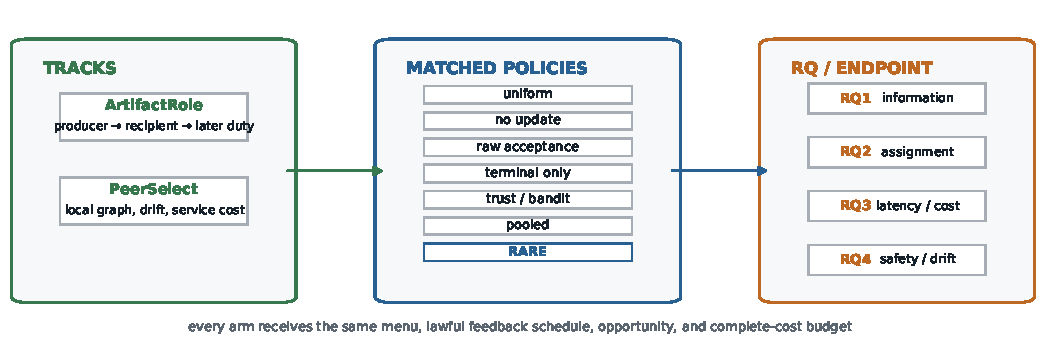
\includegraphics[width=\textwidth]{figures/experiment_map.pdf}
\caption{实验地图。ArtifactRole 测量情境化产出方--接收方现象；PeerSelect 隔离局部选择、漂移和服务成本。所有策略臂在四个研究问题评分前都获得相同的候选菜单、合法反馈计划、任务机会和完整成本预算。}
\Description{三面板地图从 ArtifactRole 和 PeerSelect 轨道出发，经过匹配的策略臂，连接到四个研究问题终点：信息、分派、延迟与成本，以及安全与漂移。}
\label{fig:experiment-map}
\end{figure*}

表~\ref{tab:headline} 预留确认清单完成后承载论文标题性比较的终点。
\begin{table}[t]
\centering\small
\caption{标题性终点。只有冻结的确认清单才能提供数值；区间为流级 95\% 区间。}
\label{tab:headline}
\begin{tabular}{p{.28\columnwidth}p{.17\columnwidth}p{.17\columnwidth}p{.17\columnwidth}}
\toprule
终点 & RARE & 最佳同信息实验臂 & 差异/区间 \\
\midrule
未来质量 & \blank & \blank & \blank \\
完整成本 & \blank & \blank & \blank \\
质量--成本效用 & \blank & \blank & \blank \\
分派改变 & \blank & \blank & \blank \\
判断 Brier 分数 & \blank & \blank & \blank \\
更新 p95 / 状态字节数 & \blank & \blank & \blank \\
旧结构根遗忘 & \blank & \blank & \blank \\
UNKNOWN / 错误归因 & \blank & \blank & \blank \\
\bottomrule
\end{tabular}
\end{table}

\subsection{预算、统计与报告}
每次模型请求在派发前预留尝试次数、提示词 token、最大生成 token、工具时间和存储；错误只释放未使用的预留资源，并保留已经观察到的成本。我们计入产出方执行、接收方集成、判断服务、通信、重试、重放、验证和返回产出物的成本。开发/搜索成本与部署成本分开报告。汇总控制器获得相同的总容量；不使用判断的实验臂仍支付声明的比较成本，或者使用共享判断调用但屏蔽其输出。

对每条流，我们记录配置、模型路由和版本元数据、代码和数据摘要、种子、硬件、时间戳、原始 API 响应、token 使用量、中间动作、失败轨迹、\unknown{} 原因和逐样本结果。我们报告带流级 95\% 区间的均值和中位数、预注册对比的效应量、各结构根的异质性、ITT 和按方案分析的分母，以及质量--成本 Pareto 点。主要终点是分派层面的未来质量--完整成本效用；源产出方分数是辅助指标，不能替代它。

对于每一个主要对比，实验卡片在确认实验前固定方向、最小实际重要差异或精度目标、流级 95\% 区间和停止规则。缺少这些字段的行只是设计规范，不能被解释为结果。

\subsection{消融与证伪}
最小消融网格为：（A）无证据/无更新；（B）只有公共证据，持久化状态不变；（C）只有延迟更新，没有新公共证据；（D）公共证据加延迟更新。额外干预一次去掉责任过滤、仅选中项限制、延迟、局部性、修正/重放或绑定分派的机制，同时固定信息、模型、候选菜单和预算。改变一条可见判断而保持终局质量不变的内容突变，应当在真正消费该判断的比较器中改变分数。

如果证据发布隐式改变了持久化策略；如果接收方修复被计入产出方；如果分派或读取截点顺序无效；如果未知或重复事件改变状态；如果情境信任解释了完整效果；或者如果在匹配完整成本下收益消失，则撤回主要主张。无效、权衡或有条件的协议结果都是科学上有效的，但不能写成成功的角色形成。

\paragraph{阶段规则。} 在选择之前，策略只能看到候选菜单、公共记录水位、读取截点摘要和封存的选择概率；隐藏金标准、未执行候选结果和未来目标结果均不可用。在责任判断阶段，记录包含判断、动作、责任所有者、改变的路径、所有权门以及明确的 \unknown{} 原因。在分派封存之后，只有相匹配的目标质量/成本事件可以产生一次仅选中项更新；没有修正谱系的迟到或重复事件不构成新标签。

\subsection{执行与结果填写契约}
剩余经验工作按照冻结的实验卡片组织，而不是开放式搜索。每张卡片命名一个矩阵行、一个结构根或 PeerSelect 流、一个策略配置和一个种子集合。派发前，卡片记录候选菜单、读取截点规则、反馈延迟、模型和编码器版本、提示词或特征模式、探索下限、更新规则、token 和墙钟预算、停止规则以及主要估计量。第一次确认调用后，这些字段不可变。失败调用仍然是一次带观察成本的尝试；它不会创建新种子，也不会悄悄把行移动到更便宜的条件。

结果填写过程有四个检查点。第一，原始账本检查器验证摘要、事件顺序、仅选中项资格以及选择时不存在未来字段。第二，评分器在不使用策略专属后处理的前提下，生成逐事件标签、\unknown{} 原因、成本和流标识。第三，分析脚本从同一清单计算预先声明的估计量和流级不确定性，写出机器可读结果对象与人类可读审计记录。第四，论文集成器只把已验证字段映射到对应表格单元和解释句子。当卡片不完整、结构根未通过资格验证或终点未定义时，单元保持 \textsc{tbd}。集成器不会把缺失值替换为零，也不会为了符合预期方向而编辑原始结果。

\begin{table}[t]
\centering\scriptsize
\setlength{\tabcolsep}{2.5pt}
\caption{确认卡片使用的结果录入规则。表格是写作契约，不是观察结果。}
\label{tab:result-contract}
\begin{tabular}{p{.18\columnwidth}p{.34\columnwidth}p{.32\columnwidth}}
\toprule
检查点 & 必需产物 & 论文允许填写的内容 \\
\midrule
资格验证 & 结构根、材料、评分器、可见性和重放检查 & 合格、探索性或 \unknown{} \\
执行 & 不可变事件账本和原始 API/工具轨迹 & 尝试次数、失败和成本 \\
分析 & 每流估计量、区间和分母 & 只有卡片完整时才能填写数值 \\
集成 & 与摘要绑定的结果对象和审查记录 & 表格单元加与证据匹配的文字 \\
\bottomrule
\end{tabular}
\end{table}

该契约也规定负面证据的写法。无效对比就报告为无效对比；没有效用收益的安全改善就报告为安全结果；能够预测却没有改变未来分派的判断，不能称为角色形成。这样，最终论文不需要在“成功故事”和“调试报告”之间事后选择：矩阵、分母和证伪规则会决定哪一项主张能够保留下来。

\section{结果与证据边界}
\label{sec:current}

\textbf{RQ1--RQ2（信息与分派）。} 确认卡片将在表~\ref{tab:headline} 和表~\ref{tab:matrix} 中填写留出集 Brier 分数、匹配信息比较、分派改变率以及未来质量--成本效用：\textsc{tbd}。没有封存的未来分派时，预测结果只能支持信息主张；没有独立目标结果时，分派结果不能证明责任转移。

\textbf{RQ3--RQ4（服务与安全）。} 延迟、积压、状态规模、遗忘、\unknown{} 和错误归因单元仍为 \textsc{tbd}。我们会把安全的无效结果、质量--成本权衡和有条件的正向结果解释为不同的主张，而不会把它们当成同一种证据。

当前真实追踪只验证工程边界。两条有限的真实 API 闭环记录了源选择、接收方判断、消费者执行、源状态快照和后续分派。两个消费者都修改了自己的集成文件，而单独的产出方审计发现了优先级产出物的失败；因此，原始消费者分数没有测量产出方正确性。反馈映射与先验相同，所以概率没有变化。这些追踪推动了责任门和审计设计，但没有证明专业化、预测、未来质量或实时训练。智能体使用的是一次新的提示，没有持久化的个体经验；任何结果单元都没有从这些回执中填写。没有合格结构根、独立流、完整成本和公平适配器的结果，仍然只能算探索性结果。

\section{讨论与局限}

本文有意把机制限制在一个比“智能体获得一般技能”或“工作流自动发现专家”更窄的范围内。研究对象是具有真实产出方--接收方依赖的任务中的责任机会。PeerSelect 可以隔离局部在线选择和漂移，但不能替代 ArtifactRole 证据。反过来，ArtifactRole 结果也不能被合并为一般老虎机收益。

主要威胁包括判断错误、选择性暴露、结构根依赖、责任覆盖不完整，以及接收方观察带来的成本膨胀。设计通过测量判断可靠性和选择倾向、保留 \unknown{} 记录并使用独立结构根和流来应对这些威胁。它不能从单一工作流家族推断普适角色语义。如果公共证据过于稀疏，正确结果可能是一个校准良好的无效结论，或者一个更窄的、任务条件化的结果。

最终骨干网络和更新器仍然开放。只有在合格轨道和强同信息基线暴露出瓶颈之后，才会选择最终方案。冻结表示加小型增量头、RLS 或在线逻辑回归、周期性重拟合和有界候选更新器都是比较条件。只有在测量到真实的更新或表示瓶颈，并且实验卡片固定挑战者、预算和确认划分之后，才有理由进行大规模 GPU 运行。

部署边界同样明确。选择器可以拒绝从含糊交接中学习，但必须把拒绝暴露给操作员，并保存事件供后续审计。选择器可以使用局部候选图，但局部性必须作为卡片字段，而不能成为未报告的优势来源。选择器可以压缩旧证据，但压缩必须保留源标识、有效区间和重建决策所需的状态摘要。这些要求使方法可以兼容工具选择服务和同行选择服务，同时保持二者的标签分离：工具结果可以由执行预言机检查，而同行判断必须通过产出方--接收方所有权门。因而，共享实现的是事件和重放层，而不是共享的真实标签。这个区别对最终主张很重要。如果实现提供低延迟更新，却无法在合格基准中识别产出方责任，我们就报告可执行的基础设施结果，并撤回角色学习主张。如果归因安全，但选择器没有改善未来分派，我们就报告校准后的证据协议，而不是自我进化。两种结果都已预先规定，并且都能为后续系统提供有用信息。

产物发布遵循同样的分离原则。代码、任务结构根、提示词、评分器版本和环境锁通过清单发布，清单把每个聚合结果指向原始事件文件。清单记录被排除的尝试及其原因，使读者能够区分“缺少结构根”和“结果为零”。重放命令可以在不联系模型提供方的情况下重建读取截点和分派封存；要复现 API 延迟和 token 成本，则必须使用单独的在线命令。我们还会发布精确的表格生成脚本和卡片级决策日志。这些细节属于科学对象，因为在线角色主张无法与证据变得可见的顺序分开。它们让审稿人能够检验同一流的正面和负面解释。

\section{结论}

本文为自我进化的多智能体角色定义了一个精确对象：接收方的情境化判断成为责任安全证据，该证据在执行前改变未来分派，而后续分派依据未见过的质量和完整成本进行评价。协议使每一条箭头都可审计，并让接近的替代方案获得相同的信息和预算。当前稿件记录了方法契约、基准和基线矩阵、统计计划以及证伪边界，同时保留空的经验单元。决定性结果将是：在不牺牲归因安全、在线服务、稳定性和成本的前提下，完整闭环是否能够超越同等信息替代方案，改善未来责任分配。

\begingroup
\sloppy
\bibliographystyle{ACM-Reference-Format}
\bibliography{references}
\endgroup
\end{document}
